\section{Background}%
\label{sec:background}


Wikidata~\cite{Vrandecic-D-2014} is a sister project of Wikipedia and it's also one of largest bases of structured knowledge on the Web.
%%
Although we have been using the term ``Wikidata data model'', the data model used by Wikidata actually comes from Wikibase, which is the open-source framework underlying Wikidata.
%%
Wikibase is a project of its own.
%%
It can be used to create other knowledge bases following the same data model as Wikidata but with different content and purposes~\cite{Diefenbach-D-2021}.


\subsection{Wikibase Data Model}%
\label{sec:background:data-model}


Wikibase's data model~\cite{Wikibase-DataModel}
%%
%\footnote{\url{https://www.mediawiki.org/wiki/Wikibase/DataModel}}
%%
consists of entities and statements about entities.
%%
In Wikidata's UI, statements are grouped into ``entity pages''.
%%
Figure~\ref{fig:benzene} shows the page of entity Q2270, which stands for the chemical compound benzene.\footnote{\url{https://www.wikidata.org/wiki/Q2270}}
%%
Every entity has a label, a description, and one or more aliases.
%%
In Figure~\ref{fig:benzene}, these are shown in the header at the top of the page.


\begin{figure}[ht]
  \centering
  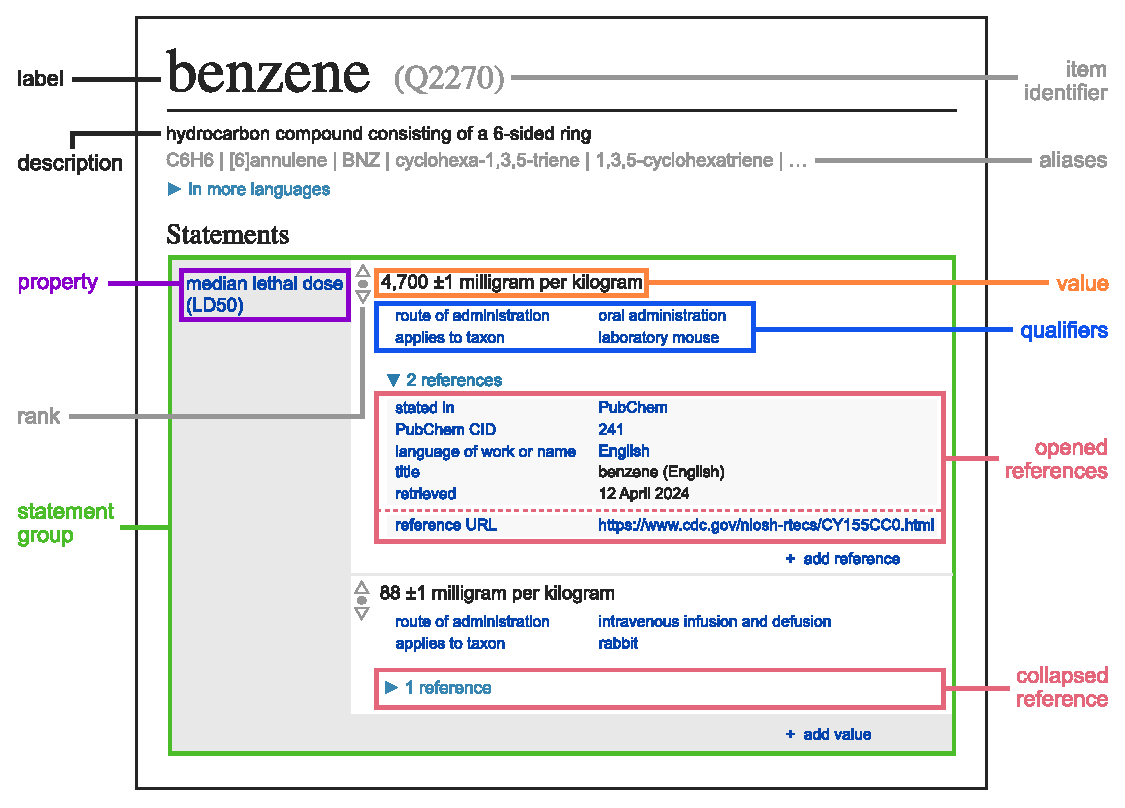
\includegraphics[width=.95\textwidth]{figs/benzene.eps}%
  \caption{Part of Wikidata's entity page of benzene. (Adapted from~\cite{Odell-J-2022}.)}%
  \label{fig:benzene}
  \vskip-.75\baselineskip%
\end{figure}


After the header comes the ``Statements'' section which groups statements about the entity being described.
%%
A \emph{statement} consists of two parts: subject and snak.
%%
The \emph{subject} is the entity about which the statement is made.
%%
The \emph{snak} is the statement's claim.
%%
It associates a property with either a specific value, some unspecified value, or no value.


Figure~\ref{fig:benzene} depicts two statements which can be read as follows:
%%
\begin{align}
  \label{eq:stmt1}
  &\text{``benzene has an LD50 of 4{,}699--4{,}701 milligrams per kilogram''}\\
  \label{eq:stmt2}
  &\text{``benzene has an LD50 of 87--89 milligrams per kilogram''}
\end{align}
%%
LD50 (or median lethal dose) is a toxicity unit that measures the dose of a substance that is required to kill half the members of a tested population.


The subject of statements~\eqref{eq:stmt1} and~\eqref{eq:stmt2} is the same, ``benzene'' (Q2270).
%%
Their snak is of the form property-value.
%%
The property of both is ``median lethal dose (LD50)'' (P2240).
%%
The value of~\eqref{eq:stmt1} is ``4{,}700 $\pm$1 mg/kg'' and the value of~\eqref{eq:stmt2} is ``88 $\pm$1 mg/kg''.
%%
Note that the data model distinguishes between items (identified with ``Q'') and properties (identified with ``P'').
%%
Only the latter can occur as the first component of snaks.


In Python, using the KIF constructors (see Figure~\ref{fig:grammar}), statements~\eqref{eq:stmt1} and~\eqref{eq:stmt2} are written as follows:
%%
\newcommand*\X[1]{$\langle\text{\scriptsize{\textrm{#1}}}\rangle$}%
\begin{pyconcode}
>>> stmt1 = Statement(Item(!\X{benzene}!),
...    ValueSnak(Property(!\X{LD50}!), Quantity(4700, !\X{mg/kg}!, 4699, 4701)))

>>> stmt2 = Statement(Item(!\X{benzene}!),
...    ValueSnak(Property(!\X{LD50}!), Quantity(88, !\X{mg/kg}!, 87, 89)))
\end{pyconcode}
%%
We write $\langle{x}\rangle$ for the URL of entity $x$, e.g., $\langle\text{benzene}\rangle$ stands for \url{http://www.wikidata.org/entity/Q2270}.


Back to Figure~\ref{fig:benzene}, the qualifiers and references associated with each statement are shown below the statement's value (see the boxes ``qualifiers'' and ``opened references'').
%%
\emph{Qualifiers} are extra snaks which qualify what is being said by the statement's main snak; \emph{references} (or \emph{reference records}) are sets of snaks which keep provenance information.


The qualifiers of statement~\eqref{eq:stmt1} shown in Figure~\ref{fig:benzene} are written as follows:
%%
\begin{pyconcode}
>>> qualifiers_of_stmt1 = [
...    ValueSnak(Property(!\X{route of administration}!), Item(!\X{oral administration}!))
...    ValueSnak(Property(!\X{applies to taxon}!), Item(!\X{laboratory mouse}!))]
\end{pyconcode}
%%
Note that the qualifiers in this case convey information that is crucial to interpret the statement, namely, the route of administration and the affected animal.


The references shown for statement~\eqref{eq:stmt1} in Figure~\ref{fig:benzene} are written as follows:
%%
\begin{pyconcode}
>>> references_of_stmt1 = [
... ReferenceRecord(    # 1st reference
...    ValueSnak(Property(!\X{stated in}!), Item(!\X{PubChem}!)),
...    ValueSnak(Property(!\X{PubChem CID}!), String('241')),
...    ValueSnak(Property(!\X{language of work or name}!), Item(!\X{English}!)),
...    ValueSnak(Property(!\X{retrieved}!), Time('2024-04-12'))),
... ReferenceRecord(    # 2nd reference
...    ValueSnak(Property(!\X{reference URL}!), IRI('http://www.cdc.gov...')))]
\end{pyconcode}


\begin{figure}[ht]
  \newcommand*\xcode[1]{\text{\code{#1}}}
  \newcommand*\NT[1]{\ensuremath{\text{\emph{#1}}}}%
  \newcommand*\EQ{\mathord{::=}}%
  \begin{mdframed}%
  \abovedisplayskip=-.5em
  \belowdisplayskip=-.5em
  %\setlength{\jot}{1.6pt}
  \def\arraystretch{1.25}
  \begin{equationarray*}{rll}%
    \NT{stmt}      \ \EQ &\ \xcode{Statement(!\NT{entity}!, !\NT{snak}!)}
                         &\text{--- claim about \NT{entity}}\\
    %%
    \NT{entity}    \ \EQ &\ \NT{item} \mid \NT{property}\\
    %%
    \NT{item}      \ \EQ &\ \xcode{Item(!\NT{iri}!)}
                         &\text{--- person or thing}\\
    %%
    \NT{property}  \ \EQ &\ \xcode{Property(!\NT{iri}!)}
                         &\text{--- (binary) relation}\\
    %%
    \NT{snak}      \ \EQ &\ \xcode{ValueSnak(!\NT{property}!, !\NT{value}!)}
                         &\text{--- ``\NT{property} has \NT{value}''}\\
                         %%
                   \ \mid&\ \xcode{SomeValueSnak(!\NT{property}!)}
                         &\text{--- ``\NT{property} has some value''}\\
                         %%
                   \ \mid&\ \xcode{NoValueSnak(!\NT{property}!)}
                         &\text{--- ``\NT{property} has no value''}\\
    %                      %%
    \NT{value}     \ \EQ &\ \NT{entity} \mid \NT{data-value}\\
    %%
    \NT{data-value}\ \EQ &\multicolumn{2}{l}{%
      \ \NT{iri} \mid \NT{text} \mid \NT{string} \mid
      \NT{external-id} \mid \NT{quantity} \mid \NT{time}}\\
                         %%
    \NT{iri}       \ \EQ &\ \xcode{IRI(!{$s$}!)}
                         &\text{--- IRI}\\
                         %%
    \NT{text}      \ \EQ &\ \xcode{Text(!{$s$}!, !\NT{lang}${?}$!)}
                         &\text{--- text in a given language}\\
                         %%
    \NT{string}    \ \EQ &\ \xcode{String(!{$s$}!)}
                         &\text{--- string}\\
    \NT{external-id}\ \EQ&\ \xcode{ExternalId(!{$s$}!)}
                         &\text{--- external id}\\
    %                      %%
    \NT{quantity}  \ \EQ &\
                   \xcode{Quantity(!{$n$}!, !\NT{item}$?$!, !{$n?$}!, !{$n?$}!)}
                         &\text{--- numerical quantity}\\
                         %%
    \NT{time}      \ \EQ &\
                   \xcode{Time(!{$ts$}!, !{$i?$}!, !{$i?$}!, !\NT{item}$?$!)}
                         &\text{--- date or time}\\
                         %%
    \NT{reference} \ \EQ&\ \xcode{ReferenceRecord(!\NT{snak}$+$!)}\\
    \NT{rank}      \ \EQ&\ \xcode{Preferred} \mid \xcode{Normal} \mid
                             \xcode{Deprecated}
  \end{equationarray*}%
  \end{mdframed}%
  \caption{Constructors of data model objects in KIF\@.  ``${?}$'' means zero-or-one; ``$+$'' means one-or-more; $s$ is a Python string; $\NT{lang}$ is a Python string containing language tag such as ``en''; $n$ is a number; $i$ is an integer; and $ts$ is a date-time timestamp.}%
  \label{fig:grammar}%
  %\vskip-1em
\end{figure}



%%% Local Variables:
%%% mode: latex
%%% TeX-engine: xetex
%%% TeX-master: "../main"
%%% eval: (visual-line-mode 1)
%%% End:



The last piece of metadata associated with statements is the \emph{rank} which can be either ``preferred'', ``normal'', or ``deprecated''.
%%
In Figure~\ref{fig:benzene}, the rank is represented symbolically by the two triangles and circle which occur on the left of the statement's value.
%%
A filled upper triangle means preferred rank; a filled circle means normal rank; and a filled lower triangle means deprecated rank.
%%
As can be seen in Figure~\ref{fig:benzene}, statements~\eqref{eq:stmt1} and~\eqref{eq:stmt2} have normal rank.


\subsection{Wikidata RDF Encoding}%
\label{sec:background:rdf}


Wikidata defines an RDF encoding for its data model which is also adopted by Wikibase~\cite{Wikibase-RDF-Dump-Format,Westerinen-A-2024}.
%%
%\footnote{\url{https://www.mediawiki.org/wiki/Wikibase/Indexing/RDF_Dump_Format}}
%%
The format varies slightly depending on whether it is used in a data dump or observed from Wikidata's query service.
%%
The version we describe here is that of the query service.


In Wikidata's RDF encoding, each statement is represented at two levels.
%%
The first level, called \emph{truthy}, keeps a shallow representation of the statement as a single RDF triple.
%%
For example, the truthy encoding of statement~\eqref{eq:stmt1} of Figure~\ref{fig:benzene}, namely, ``benzene (Q2270) has an LD50 (P2240) of 4{,}700$ \pm$1 mg/kg'', consists of the single triple:
%%
\begin{equation}
\label{eq:benzene-truthy}
\begin{tikzpicture}[node distance=6em,baseline]
  \node[n,draw](benzene){\strut\text{wd:Q2270}};
  \node[l,right=of benzene](value){\strut\text{"4700"{\^{}\^{}xsd:decimal}}};
  \draw[->] (benzene) -- node[e,above,inner sep=2pt]{wdt:P2240} (value);
\end{tikzpicture}\tag{$\dagger$}
\end{equation}


%%% Local Variables:
%%% mode: latex
%%% TeX-engine: xetex
%%% TeX-master: "../main"
%%% eval: (visual-line-mode 1)
%%% End:

%%
The namespace \code/wd:/ indicates an entity and \code/wdt:/ indicates a truthy application of a property.
%%
Some statements are fully characterized at the truthy level.
%%
But, as illustrated by~\eqref{eq:benzene-truthy}, this is not always the case.
%%
Note that the unit, lower-, and upper-bounds associated with the value 4700 are not represented in~\eqref{eq:benzene-truthy}.
%%
In general, when the statement's value is a structured data-value, like a quantity or time value, a single literal is used to represent it at the truthy level.
%%
This is the so called \emph{simple value} of the statement.
%%
For quantity values, the simple value is is just the numerical amount.


%%
% TODO: Explain that, i.e., the first argument of the \code/Quantity/ constructor.
%%


The second level of the encoding keeps the full representation of the statement.
%%
It uses reification to capture the \emph{deep value} of the statement plus its qualifiers, references, and rank.
%%
Figure~\ref{fig:benzene-deep} depicts the full representation of statement~\eqref{eq:stmt1} of Figure~\ref{fig:benzene} considering only one qualifier and one reference record.


\begin{figure}[ht]
  \vskip-\baselineskip%
  \centering
  \begin{tikzpicture}[s/.style={n,fill=gray!25},node distance=4em and 4em]
    \node[s](wds){\strut\code/wds:_/};
    \node[n,above left=of wds](benzene){\strut wd:Q2270};
    \node[l,above right=of wds](value){\strut "4700"\rlap{\^{}\^{}xsd:decimal}};
    \draw[->](benzene) to node[e]{wdt:P2240} (value);
    \draw[->](benzene) to[bend right=10] node[e,above]{p:P2240} (wds);
    %%
    \begin{scope}
      \node[n,left=of wds,xshift=-2em,text width=6em,align=center]
      (NormalRank){\strut wikibase:\\[-2pt]\strut NormalRank};
      \draw[->](wds) to node[e,text width=3.5em,align=center]
      {wikibase:\\[-2pt]rank} (NormalRank);
    \end{scope}
    \draw[->](wds) to[bend right=10] node[e,above]{ps:P2240} (value);
    %%
    \node[s,below right=of wds](wdv){\strut\code/wdv:_/};
    \draw[->](wds) to[bend left=10] node[e,below,yshift=1pt]{psv:P2240} (wdv);
    \draw[->](wdv) to[bend left=10]
    node[e,text width=6em,align=center,yshift=.5em]
    {wikibase:\\[-2pt]quantityAmount} (value);
    %%
    \node[n,above right=of wdv,text width=7em,align=center,yshift=1em]
    (QuantityValue){\strut wikibase:\\[-2pt]\strut QuantityValue};
    \draw[->](wdv) to[bend left=10]node[e]{rdf:type} (QuantityValue);
    %%
    \node[n,right=of wdv,xshift=3em,yshift=2em](Unit){\strut wd:Q21091747};
    \draw[->](wdv) to[bend left=10]
    node[e,text width=4.7em,align=center,yshift=-.3em]
    {wikibase:\\[-2pt]quantityUnit}(Unit);
    %%
    \node[l,below right=of wdv,yshift=2em](LB)
    {\strut"4699"\rlap{\^{}\^{}xsd:decimal}};
    \draw[->](wdv) to[bend right=10] node[e,align=center,xshift=4em,yshift=.4em]
    {wikibase:quantityLowerBound}(LB);
    %%
    \node[l,below=of wdv=0em,xshift=-1em](UB)
    {\strut "4701"\rlap{\^{}\^{}xsd:decimal}};
    \draw[->](wdv) to[bend right=10]
    node[e,align=center,text width=7em,xshift=-2em]
    {wikibase:quantity\\[-2pt]UpperBound}(UB);
    %%
    \node[n,below=of wds](Oral){\strut wd:Q285166};
    \draw[->](wds) to[bend right=10] node[e]{pq:P636}(Oral);
    %%
    \node[s,below left=of wds](wdref){\strut\code/wdref:_/};
    \node[n,below=of wdref](refurl)
    {\strut https://www.cdc.gov/...};
    \draw[->](wds) to[bend right=10] node[e,below,yshift=1pt,xshift=-3em]
    {prov:wasDerivedFrom} (wdref);
    \draw[->](wdref) to[bend right=10] node[e]{pr:P854} (refurl);
  \end{tikzpicture}
  \caption{RDF representation of the statement ``Benzene (Q2270) has an LD50 (P2240) of 4{,}700 $\pm$1 mg/kg (Q21091747)'' considering only the qualifier ``route of administration (P636) is oral administration (Q285166)'' and the reference record ``reference URL (P854) is \url{https://www.cdc.gov/niosh-rtecs/CY155CC0.html}''.}%
  \label{fig:benzene-deep}%
  \vskip-1.5\baselineskip%
\end{figure}


%%% Local Variables:
%%% mode: latex
%%% TeX-engine: xetex
%%% TeX-master: "../main"
%%% eval: (visual-line-mode 1)
%%% End:



In Figure~\ref{fig:benzene-deep}, the shaded nodes are the reified ones.
%%
The single underscore~(\code/_/) indicates that their ids are opaque (hence not shown in the figure).
%%
Node \code/wds:_/ represents the statement.
%%
Predicates \code/p:P2240/ and \code/ps:P2240/ are used to connect the subject ``benzene'' (\code/wd:Q2270/) to the statement and the statement to its simple value, i.e., the number 4700 in decimal notation.

The deep value of the statement is represented by node \code/wdv:_/.
%%
It has type \code/wikibase:QuantityValue/ and is connected to the unit mg/kg (\code/wd:Q21091747/), the lower-bound 4699, and the upper-bound 4701.
%%
The rank of the statement is connected via predicate \code/wikibase:rank/.

Moving to qualifiers, predicate \code/pq:P636/ connects the qualifier ``route of administration'' (P636) with value ``oral administration'' (\code/wd:Q285166/) to the statement.
%%
Finally, predicate \code/prov:wasDerivedFrom/ connects to the statement the reference record represented by node \code/wdref:_/.
%%
Its content (the snak ``reference URL'' (P854) with value ``\code|https://www.cdc.gov/...|'') is encoded using predicate \code/pr:P854/ and a (simple) IRI value.


% LocalWords:  Wikibase Wikibase's UI snak LD snaks KIF IRI eq stmt truthy
% LocalWords:  wd wdt



%%% Local Variables:
%%% mode: latex
%%% TeX-engine: xetex
%%% TeX-master: "main"
%%% eval: (visual-line-mode 1)
%%% End:
